\label{capitolo1}
\section{Introduzione}
A partire dalla metà degli anni '80, grazie a due innovazioni tecnologiche si fecero diversi passi avanti nell'uso dei calcolatori. La prima di queste innovazioni fu lo sviluppo di microprocessori potenti; la seconda grande innovazione fu l'invenzione delle reti di computer con l'introduzione delle \textbf{LAN} (\emph{Local Area Network}) che consentirono a centinaia di macchine di essere connesse le une alle altre e permisero lo scambio di piccole quantità di informazioni in pochi microsecondi.\\
Il risultato di questa innovazione tecnologica è che oggi mettere insieme una grande quantità di computer tramite una rete ad alta velocità è diventato molto semplice. Questo tipo di sistemi sono solitamente chiamate \emph{reti di computer} o \textbf{sistemi distribuiti}.
\subsection{Definizione di sistema distribuito}
Esistono diverse definizioni di \emph{Sistema distribuito} ma tutte quante sono abbastanza insoddisfacenti. Daremo ora una prima definizione che è sufficente per i nostri scopi:
\begin{center}
\emph{Un sistema distribuito è una collezione di computer indipendenti che appare ai propri utenti come un singolo sistema coerente}
\end{center}
Da questa definizione possiamo ricavare diversi caratteristiche di un sistema distribuito, la prima è che i sistemi distribuiti sono costituiti da componenti autonomi; la seconda è che gli utenti, siano essi persone o altri programmi, vedono il sistema come un'unica entità. Il che significa che i diversi componenti devono in qualche modo collaborare.\\
Quello che non viene specificato in questa definizione è il tipo di computer usati per i componenti ne come questi sono interconnessi.\\
Le caratteristiche più importanti dei sistemi distribuiti sono il fatto che le differenze tra i vari computer e le loro modalità di comunicazione risultano per lo più nascoste agli utenti finali. Inoltre gli utenti possono interagire con un sistema distribuito in modo \emph{consistente} e \emph{uniforme} ovvero indipendentemente da dove e quando avviene l'interazione.\\
Teoricamente i sistemi distribuiti dovrebbero essere facilmente espandibili e scalabili, inoltre, i sistemi distribuiti sono di norma sempre disponibili anche se alcune sui parti sono momentaneamente fuori uso.\\
Allo scopo di supportare reti eterogenee e sistemi operativi differenti alle volte si introduce uno strato software tra lo strato di applicazione e i diversi sistemi operativi, questo strato è chiamato \textbf{middleware} come mostrato in figura \ref{fig:midd}.
\begin{figure}[htb]
\centering
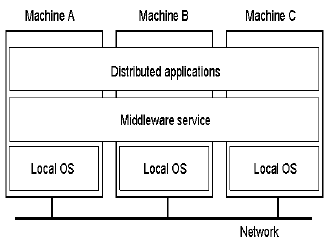
\includegraphics[width=8cm]{img/schemamidd.png}\\
\label{fig:midd}
\caption{Schema di un middleware}
\end{figure}
\subsection{Obiettivi}
La possibilità costruire sistemi distribuiti non implica che tutti i sistemi debbano essere costruiti come sistemi distribuiti. Per far si che sia utile progettare e costruire un sistema distribuito dobbiamo rispettare alcune caratteristiche. un sistema distribuito dovrebbe:
\begin{itemize}
\item rendere le risorse facilmente accessibili,
\item nascondere il fatto che le risorse sono distribuite sulla rete,
\item essere aperto,
\item essere scalabile.
\end{itemize}
\subsubsection{Accessibilità delle risorse}
L'obiettivo principale di un sistema distribuito è quello di rendere facile l'accesso alle risorse remote e condividerle in maniera efficiente e controllata.\\
Ma che cosa intendiamo per "risorse"? Con il termine \emph{risorse} possiamo indicare qualsiasi cosa, alcuni esempi tipici sono stampanti, computer, dati, file, pagine web o intere reti.
Le ragioni che portano a voler condividere le risorse sono molteplici, la prima è sicuramente quella economica, pensiamo ad esempio a ricercatori che condividono un supercomputer o ad una stampante condivisa in un ufficio. Inoltre, la connessione di più utenti facilita la collaborazione come avviene nei \textbf{groupware} dove gruppi di persone lavorano insieme anche stando in diverse parti del mondo.\\
Tutto questo incremento di connessione e collaborazione dovrebbe portare però ad una necessaria crescita anche in termini di sicurezza, anche se nella pratica attuale tale incremento nei sistemi di sicurezza non è ancora avvenuto; non è raro trovare sistemi in cui password e altre informazioni sensibili sono inviate come testo in chiaro. Altri problemi legati alla sicurezza sono l'aumento delle \emph{junk mail} o mail di \emph{spam} e l'invio e la raccolta di informazioni riguardanti l'utente per creare un profilo mentre è connesso.
\subsubsection{Trasparenza}
Uno degli obiettivi principali in  un sistema distribuito è quello di nascondere che i processi e le risorse sono distribuiti. Un sistema in grado di presentarsi come un singolo computer è detto \textbf{trasparente}.\\
Possiamo catalogare la trasparenza in diversi tipi in quanto qesto concetto può riguardare molti aspetti di un sistema distribuito.\\
La \textbf{trasparenza all'accesso} riguarda le differenze nella rappresentazione dei dati e la modalità di accesso alle risorse da parte degli utenti. Ovvero si desidera nascondere le differenze nelle macchine e trovare un accordo nella rappresentazione dei dati.
Un altro importante tipo di trasparenza è la \textbf{trasparenza di ubicazione} che si prefigge l'obiettivo di nascondere agli utenti la localizzazione di una risorsa. I \emph{nomi} in questa tipo di trasparenza giocano un ruolo importante in quanto è possibile raggiungere tale trasparenza assegnando ad ogni risorsa un nome logico indipendente dalla sua locazione, un esempio di tale tecnica sono gli \emph{URL}.\\
Alcuni sistemi distribuiti che consentono lo spostamento delle risorse senza compromettere la possibilità di accesso devono fornire la \textbf{trasparenza alla migrazione}. Nel caso in cui le risorse possono essere spostate \emph{durante} l'utilizzo senza che utenti o applicazioni notino tale spostamento si deve garantire anche la \textbf{trasparenza al riposizionamento}.\\
La \textbf{trasparenza alla replica} riguarda la possibilità di fornire una o più copie della stessa risorsa per aumentarne la disponibilità e migliorare le prestazioni, tutto questo nascondendo all'utente il fatto che la risorsa è replicata.\\
Come già detto l'obiettivo principale dei sistemi distribuiti è la condivisione di risorse, ma questa porta in alcuni casi ad avere una condivisione di tipo \emph{competitivo} ovvero, più utenti vorrebero accedere alle stesse risorse (es. una tabella di un database) tutto ciò deve essere evitato tramite la \textbf{trasparenza alla concorrenza} che deve lasciare la risorsa in uno stato consistente. Questa consistenza può essere ottenuta tramite diverse meccanismi tra cui ad esempio il \emph{locking} nel quale gli utenti ottengono a turno l'accesso esclusivo ad una risorsa.\\
Per introdurre l'ultimo tipo di concorrenza partiamo da un'altra definizione di sistema distribuito
\begin{center}
\emph{Ne apprendi l'esistenza quando il crash di un computer di cui non hai mai sentito parlare ti impedisce di portare a termine qualunque lavoro}
\end{center}
Questa definizione pone un altro aspetto importante della progettazione di un sistema distribuito, quello della gestione dei guasti; rendere un sistema \textbf{trasparente ai guasti} significa far si che un utente non si renda conto che una risorsa smette di funzionare correttamente. La difficoltà più grande è distinguere quando una risorsa è morta da quando è semplicemente molto lenta.\\
Sebbene in generale si preferisce avere sistemi trasparenti ci sono situazioni in cui nascondere completamente agli utenti la distribuzione del sistema non è una buona idea. Come nel caso si voglia contattare un servizio che sta dall'altra parte del mondo e si voglia una risposta in un tempo inferiore ai 35ms; o quando si vuole che due repliche siano sempre consistenti, nel caso di server in due continenti diversi un aggiornamento potrebbe richiedere alcuni secondi.\\
Il problema principale che limita però la trasparenza è la trasparenza stessa, infatti, ammettendo che la completa trasparenza di un sistema è \emph{impossibile} è \emph{saggio} cerca di ottenerla a tutti i costi? Rendere la distribuzione esplicita può aiutare gli utenti a capire eventuali comportamenti \emph{anomali} del sistema.
\subsubsection{Apertura}
un altro obiettivo dei sistemi distribuiti è l'apertura. un sistema distribuito \textbf{aperto} è un sistema che offre servizi rispettando delle regole standar che descrivono la sintassi e la semantica dei servizi stessi.\\
Nei sistemi distribuiti i servizi sono descritti tramite \textbf{interfacce} per lo più utilizzando un linguaggio denominato \emph{IDL (interface description language)} che però descrive soltanto la sintassi delle interfacce, ovvero, il nome delle funzioni e i tipi di parametri, i valori di ritorno o le possibili eccezioni sollevate. Per la descrizione di che cosa fa il servizio, invece, si usa solitamente il linguaggio naturale.\\
Se l'interfaccia è ben specificata un processo che ha bisogno di una determinata interfaccia può comunicare con un altro processo che implementa tale interfaccia; inoltre, consente a due processi distinti di implementare tale interfaccia in due modi completamente diversi, il che porta a due sistemi distribuiti che però  operano allo stesso modo.\\
Una specifica però deve essere \emph{completa} e \emph{neutrale}, completa significa che viene specificato tutto ciò che è necessario per realizzare un'implementazione, ma ottenere la completezza è molto difficile e perciò di solito un programmatore deve aggiungere dettagli specifici dell'implementazione. Per neutrale si intende, invece, che la specifica non deve imporre dettagli sull'implementazione. Completezza e neutralità portano ad altre due importanti caratteristiche che i sistemi distribuiti dovrebbero soddisfare, \textbf{interoperabilità} che significa che due implementazioni di vendor diversi possono collaborare e coesistere basandosi unicamente su di uno standar comune. \textbf{Portabilità} indica la possibilità di eseguire un applicazione scritta per un sistema distribuito $A$ su di un sistema distribuito $B$ senza dover apportare modifiche all'applicazione.\\
Infine un altro obiettivo che i sistemi distribuiti dovrebbero prefissarsi è che l'aggiunta o la sostituzzione di componenti dovrebbe risultare facile e non influire sui componenti già presenti; questa caratteristica sta ad indicare che il sistema distribuito è \textbf{ampliabile}.